\documentclass[
  notitlepage,
  twoside,
 % twocolumn,
   prb,
  floatfix,
% preprintnumbers,
%  preprint,
% endfloats,
%  floatfix,
%  superscriptaddress,
% nofootinbib
  %draft
]{revtex4-1}


%\usepackage[T1]{fontenc}
%\usepackage[latin9]{inputenc}
%\usepackage{babel}
\usepackage{amsmath}
\usepackage{amssymb}
\usepackage{color}
\usepackage{graphicx}
\usepackage{tabularx}
\usepackage{subfigure}
\usepackage{dcolumn}
\usepackage{textcomp}
%\usepackage{bibunits}
\usepackage{units}
\usepackage{gensymb}
\usepackage{hyperref}

% commands for structuring
\newcommand{\sect}[1]{Sect.~\ref{#1}}
\newcommand{\fig}[1]{Fig.~\ref{#1}}
\newcommand{\eq}[1]{(\ref{#1})}
\newcommand{\tab}[1]{Table~\ref{#1}}
\newcommand{\tbhd}[1]{{\bf #1}}


\begin{document}

 \title{ 
 w90pov manual
}        
\author{Daniel \AA{}berg}
\date{\today}

\maketitle
This document briefly describes how to use the ray-tracing software \textsf{POV-Ray} to render isosurfaces from {\tt xsf} files generated by the program package \textsf{wannier90}. It is assumed that \textsf{POV-Ray} is already installed. Specifically, to be able to render smooth isosurfaces using tri-linear interpolation, the \textsf{POV-Ray} version number needs to be larger than 3.6 (currently it's in v3.7 RC5, binaries and sources are available at \url{http://www.povray.org/beta}). 

A working knowledge of \textsf{POV-Ray} is of course nice, but is no prerequisite. The interested reader is referred to the  \textsf{POV-Ray} official site \url{http://www.povray.org/} and Friedrich Lohmueller's tutorial on anaylical geometry, \url{http://www.f-lohmueller.de/pov_tut/a_geo/a_geo__e.htm}. Comments and/or bugs can be sent to {\tt aberg2@llnl.gov}. 

\subsection*{Compilation}
Modify {\tt Makefile} according to your installation and then type `{\tt make}'.

\subsection*{Usage}
It is recommended to create a separate directory and copy/move/link the already produced {\tt xsf} files to that directory. Edit the input file \textsf{w90pov.inp} (to be described in the next section) and then run \textsf{w90pov}:

\mbox{}\\
\indent {\tt \$> w90pov\ w90pov.inp}
\mbox{}\\

This will produce four text files as well as a number of {\tt df3} files. The latter are binary files containing the Wannier function data in a format suitable for \textsf{POV-Ray}. The text files contain all other information about the atomic structure and isosurfaces.

\begin{itemize}
\item {\tt<seedname>.pov} \\
This is the main scene file and only tells \textsf{POV-Ray} which other files to include.
\item {\tt mydefs.inc} \\
Contains information on camera, light, where to aim the camera, cell metric, as well as macros to render atoms, bonds, and isosurfaces.
\item {\tt densities.inc} \\
Contains definitions of the {\tt df3} files and the corresponding cell metric.
\item{\tt unitcell.inc} \\
Contains information on atomic positions, bonds, and colors.
\item{\tt blobs.inc} \\
Contains information which isosurface at what isolevel to render (as well as isosurface color)
\end{itemize}

Feel free to experiment with the settings in these files, specifically the camera position, zoom, where to aim the camera, and which atoms to include. Examples can be found in the {\tt examples} directory.

To render the scene then enter:

\mbox{}\\
\indent {\tt \$> povray <seedname>.pov  +H\{height\} +W\{width\} +A0.14} 
\mbox{}\\

Of course replace {\tt <seedname>} with the seedname from the \textsf{wannier90} calculation, and {\tt \{height\} and \{width\} } with the desired size of your picture. The ``{\tt +A}" option enables anti-aliasing. In addition, the output format can be controlled using ``{\tt +F}"$x$, where $x$ can take, for example, the values {\tt C} (compressed Targa-24), {\tt N} (PNG), {\tt P} (PPM), or {\tt T} (uncompressed Targa-24). The output file name can be set using ``{\tt +O<outfile>}". Please refer to the \textsf{POV-Ray} documentation for further details.


\subsection*{The {\tt w90pov.inp} file}

\begin{itemize}
\item
{\tt numwan} - integer; \\   
Number of Wannier functions to render.

\item
{\tt seedname} - character string; \\
The root name of \textsf{wannier90} files.

\item
{\tt wanlist}  - integer array; \\
List of {\tt xsf} files to read, of length {\tt numwan}.

\item
{\tt isolevel} - real array; \\ 
List of isolevels to render, of length {\tt numwan}. The allowed range {\tt (MAX,MIN)}
for a given function is shown during the run.

\item
{\tt isopm} - real array; \\
List of how to render each function, of length {\tt numwan}. \\
{\tt -1} = negative values; \\
{\tt  0} = don't render this function; \\
{\tt 1} = positive values; \\
{\tt 2} = positive and negative values.

\item
{\tt wancol} - real array; \\
 List of colors in rgb format to use for isosurfaces, of length $3\times${\tt numwan}. The values, three for each color, are assumed to range from 0-1.

\item 
{\tt trans} - real array;\\
 List of degree of transparency for each surface, of length {\tt numwan}. \\
{\tt 0} = opaque; \\
{\tt 1} = transparent.

\item 
{\tt camera} - character string; \\
Camera position. There are six choices, valid entries are {\tt x}, {\tt y}, {\tt z}, 
{\tt a1}, {\tt a2}, and {\tt a3}. In each case, the camera is positioned along the corresponding vector. By default, the camera looks at the center of the cell (see {\tt lookpos}).

\item
{\tt lookat} - real array, optional; default: center of unit cell; \\
Position where camera is aimed in Cartesian coordinates; length 3.

\item
{\tt bondcut} - real number, optional; default: {\tt 0.9}; \\
Bond cut-off prefactor. Bonds are ``drawn" if the distance between two atoms are less then the sum of their covalent radii $\times$ {\tt bondcut}. If {\tt bondcut} is negative then a bond is drawn if the distance between two atoms is smaller than the absolute value of this number.

\item
{\tt bondrad} - real number, optional; default: {\tt 0.2}; \\
Bond-radius prefactor. The radius of the bond is set to min(radius(atom1),radius(atom2)) $\times$ {\tt bondrad}.

\item
{\tt radialfactor} - real number, optional; default: {\tt 0.5}; \\
Atomic radius prefactor. Atoms are rendered with the covalent radius $\times$ {\tt radialfactor}. The covalent radii are taken from \url{http://www.ccdc.cam.ac.uk/products/csd/radii/table.php4#group} and can be found in the the subroutine {\tt write\_unitcell} of {\tt driver.f90}.

\item
{\tt interpolation} - integer number, optional; default: {\tt 2}\\
Determines the degree of interpolation of isosurface. Use {\tt 2} for production and, e.g., {\tt 1} to test the orientation of the camera. 

\item 
{\tt zoom} - real number;\\
Zoom factor. Here you have to play around. It's recommended to set {\tt isopm} to an array of zeros or set {\tt interpolation} to zero when finding to the best position and zoom.

\item 
{\tt cellim} - real array, optional; default: {\tt 0\ 1\ 0\ 1\ 0\ 1}; \\
Defines a ``box'' in which atoms are rendered. The format is \\
{\tt <a1\_min> <a1\_max> <a2\_min> <a2\_max> <a3\_min> <a3\_max>} \\
and is given in units of the Bravais lattice vectors. Thus, the default values correspond to the atoms inside the unit cell. Note that the code accepts non-integer numbers.

\item 
{\tt cutsphere} - real number, optional; no default; \\
Any atom that is located outside a sphere, centered at {\tt lookat}, having radius {\tt cutsphere} will not be rendered.

\item
{\tt lcage} - logical, optional; default: {\tt true};\\
Render the unit cell.

\item
{\tt aspectratio} - real number, optional; default: {\tt 1.0}; \\
Specifies the aspect ratio between image width and height. Be sure to use the same ratio in the actual call to \textsf{povray} (e.g. $+${\tt H}$\{x\}$ $+${\tt W}$\{x\times${\tt aspectratio}$\}$)

\end{itemize}

\subsection*{Examples}
A number of examples can be found in the {\tt examples} directory. Be sure to first \textsf{gunzip} any {\tt *.gz} files.

\begin{enumerate}
\item {\tt examples/1.PdN2\_1} \\
Rendering of four $d$-orbitals centered at Pd atoms in PdN$_2$, see \fig{apa1}.

\item {\tt examples/2.PdN2\_2} \\
Magnification of one of Pd $d$-orbitals, see \fig{apa2}. Here I've used {\tt lookpos} and {\tt cutsphere}. You will need to copy across {\tt pdn2\_00004.xsf} from example 1. Note that {\tt aspectratio} is set to {\tt 2.0}, so make sure to specify the correct ratio between the width and height when rendering (``$+${\tt H}$\{x\}$ $+${\tt W}$\{2x\}$"). 

\item {\tt examples/3.PdN2\_3} \\
Same orbital as in the last example (i.e., you will need to copy across {\tt pdn2\_00004.xsf} from example 1), but with several transparent isosurfaces (see \fig{apa3}). This was generated using the example input file, and manually editing the file {\tt blobs.inc}. So, to create multiple isosurfaces, find a line with {\tt elblob}, copy this as many times you wish, and edit the first and last number in each line. These numbers correspond to the isolevel and transparency, respectively. To render this figure, first run \textsf{w90pov}, copy {\tt blobs.inc\_more} to {\tt blobs.inc}, and run \textsf{povray}.

\item {\tt examples/4.LaBr3\_1} \\
Bromine $p$-orbital in LaBr$_3$, see \fig{apa4}.

\item {\tt examples/5.LaBr3\_2} \\
Lanthanum $f$-orbital in LaBr$_3$, see left panel in \fig{apa5}.
\item {\tt examples/6.LaBr3\_3} \\
Lanthanum $f$-orbital in LaBr$_3$, see right panel in \fig{apa5}. This represents a manual ``tweak'' of example 5. You will need to copy across the two {\tt df3} files generated in example 5. In the file {\tt mydefs.inc} you'll find a new isosurface-macro ({\tt elblob2}) that turns the ``blob'' into glass. Also, the camera-type has been changed into perspective (instead of orthographic), a plane and sky have been added, and finally the scene is rendered using photons (that is, realistic reflection/refraction). 
\end{enumerate}

\newpage
 \begin{figure}
 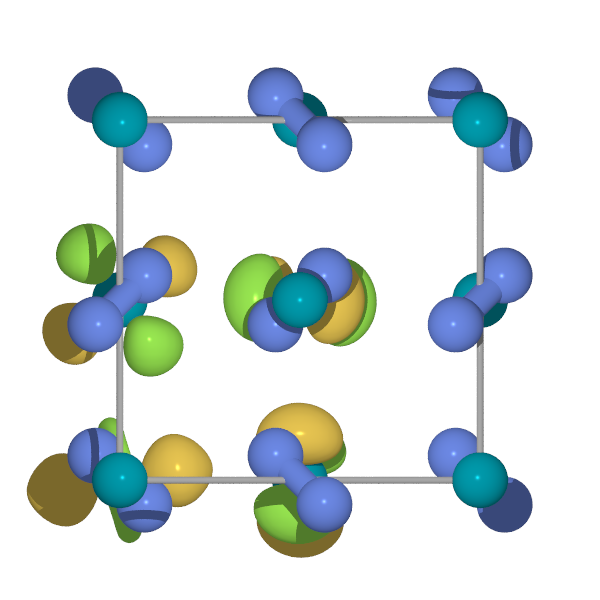
\includegraphics[width=2.0in]{figs/pdn2_1}
 \caption{Four $d$-orbitals in PdN$_2$.}
 \label{apa1}  
\end{figure}

 \begin{figure}
  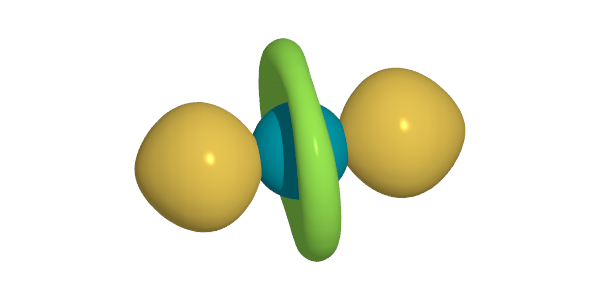
\includegraphics[width=3.0in]{figs/pdn2_2}
  \caption{One of the $d$-orbitals in PdN$_2$.}
  \label{apa2}  
 \end{figure}
  
 \begin{figure}
  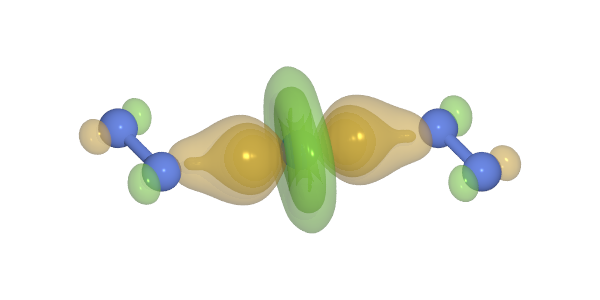
\includegraphics[width=4.0in]{figs/pdn2_3}
  \caption{One of the $d$-orbitals in PdN$_2$ with several transparent isosurfaces.}
  \label{apa3}  
 \end{figure}
 
 \begin{figure}
  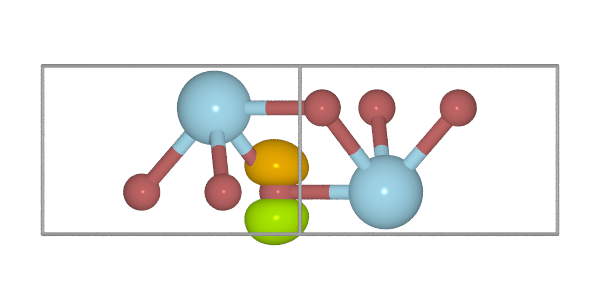
\includegraphics[width=4.0in]{figs/labr3_1}
  \caption{Bromine $p$-orbital in LaBr$_3$.}
  \label{apa4}  
 \end{figure}

 \begin{figure}
  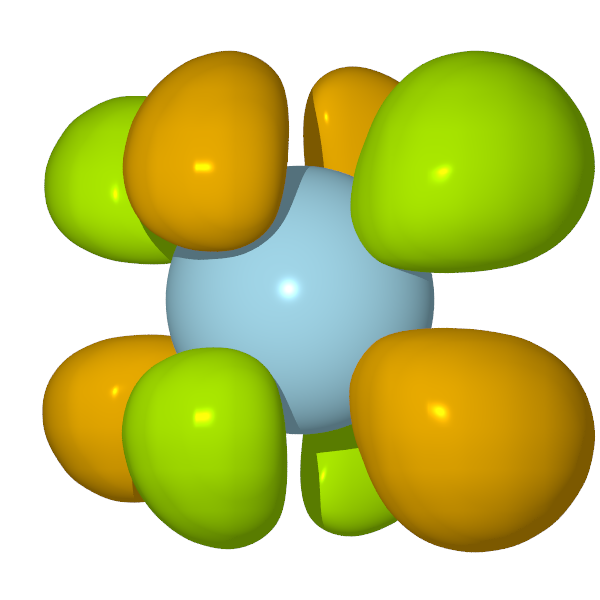
\includegraphics[width=2.0in]{figs/labr3_2}
  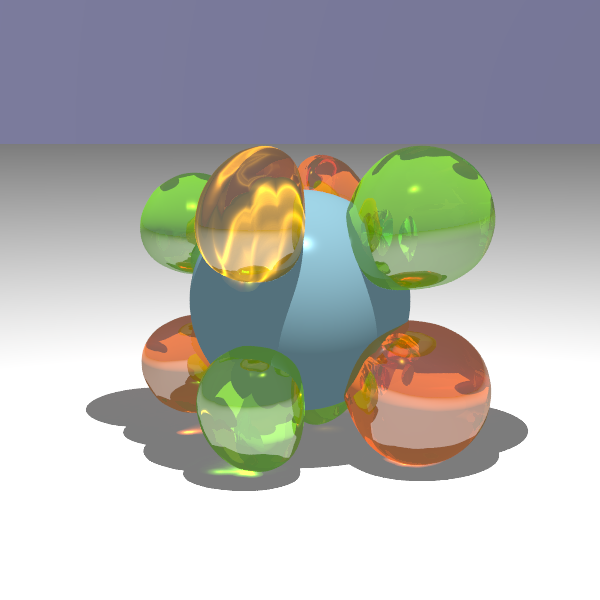
\includegraphics[width=2.0in]{figs/labr3_3}
  \caption{Lanthanum $f$-orbital in LaBr$_3$.}
  \label{apa5}  
 \end{figure}
 



\end{document}
